\documentclass[10pt,journal,compsoc]{IEEEtran}

%----------------------------------------------------------------------------------------
% PACKAGES
%----------------------------------------------------------------------------------------
\ifCLASSOPTIONcompsoc
  \usepackage[nocompress]{cite}
\else
  \usepackage{cite}
\fi

% --- Graphic & Mathematics ---
\usepackage{graphicx}
\usepackage{amsmath,amsfonts}

% --- Algorithm & Tables ---
\usepackage{algorithmic}
\usepackage{algorithm}
\usepackage{array}
\usepackage{tabularx}
\usepackage{multirow}
\usepackage{booktabs}

% --- Color & Links ---
\usepackage[dvipsnames]{xcolor} 
\usepackage[
    colorlinks=true, 
    linkcolor=blue, 
    citecolor=blue,
    urlcolor=blue
]{hyperref}

% --- Other Tools ---
\usepackage{url}
\ifCLASSOPTIONcompsoc
  \usepackage[caption=false,font=footnotesize,labelfont=sf,textfont=sf]{subfig}
\else
  \usepackage[caption=false,font=footnotesize]{subfig}
\fi

% --- Bibliography ---
\bibliographystyle{unsrt}

%----------------------------------------------------------------------------------------
% DOCUMENT BODY
%----------------------------------------------------------------------------------------
\begin{document}

\title{From NeRFs to 3D Gaussians: A Survey on Dynamic Scene Modeling and Rendering}

\author{
  Yuwei~Zhao, Kaiyuan~Zhang, Yuxiang~Liu, Yilin~Zhang, and~Keqin~Zhang%
  \IEEEcompsocitemizethanks{
      \IEEEcompsocthanksitem Y. Zhao, K. Zhang, Y. Liu, Y. Zhang, and K. Zhang are with the School of Computer Science and Technology, Ocean University of China, Qingdao 266100, China, and also with the School of MPs \& EPs, Heriot-Watt University, Edinburgh EH14 4AS, UK.
      % 通讯作者...
  }
}

%----------------------------------------------------------------------------------------
\IEEEtitleabstractindextext{
  \begin{abstract}
    Dynamic scene modeling is a pivotal technology for emerging applications in the Metaverse, virtual reality, and free-viewpoint video. While Neural Radiance Fields (NeRF) have achieved photorealistic rendering, their application to dynamic scenes is hindered by slow training and inference speeds. Recently, 3D Gaussian Splatting (3DGS) has emerged as a disruptive alternative, offering real-time rendering capabilities through explicit splatting. 
    In this survey, we provide a comprehensive review of the transition from implicit to explicit representations for dynamic scene modeling. We propose a structured taxonomy categorizing existing methods into four paradigms: Implicit Deformation Fields, Spacetime Neural Fields, Hybrid Representations, and Dynamic Gaussian Splatting. 
    Furthermore, we conduct a systematic comparative analysis based on reconstruction quality, training efficiency, and storage footprint. Our analysis reveals that while implicit methods excel in storage efficiency ($<5$ MB), explicit Gaussian-based methods demonstrate superior real-time performance ($>80$ FPS). 
    Finally, we discuss open challenges, including storage compression and integration with generative AI, outlining future directions for this rapidly evolving field.
    Our compiled resources are available at \url{https://github.com/8arbatos/Academic-English-Group-Paper}.
  \end{abstract}

  \vskip -0.1in

  \begin{IEEEkeywords}
    Dynamic Scene Modeling, Neural Radiance Fields, 3D Gaussian Splatting, View Synthesis, 4D Reconstruction.
  \end{IEEEkeywords}
}

\maketitle

%----------------------------------------------------------------------------------------
\IEEEraisesectionheading{\section{Introduction}}
\IEEEPARstart{W}{ith} the rapid advancement of virtual reality (VR), augmented reality (AR), and the Metaverse, the demand for photorealistic 3D content creation has surged exponentially. 
Dynamic scene modeling, which aims to reconstruct 3D geometry and appearance from 2D video streams, serves as a fundamental technology for these applications, enabling immersive telepresence, free-viewpoint video, and digital human avatars \cite{intro_metaverse}. 
Unlike static scene reconstruction, modeling dynamic scenes from video presents a highly ill-posed inverse problem due to the entanglement of object motion, topology changes, and time-variant lighting conditions.

Traditionally, 3D reconstruction relied on Structure-from-Motion (SfM) and Multi-View Stereo (MVS) algorithms \cite{colmap}. 
While these methods, such as COLMAP, provide robust camera pose estimation, they struggle to capture thin structures and view-dependent effects (e.g., reflections). 
More importantly, traditional pipelines typically assume a static world, making them brittle when applied to dynamic video sequences where geometry consistency is violated over time.

To address dynamic content before the deep learning era, non-rigid reconstruction methods were developed to warp a canonical template to live frames. 
Pioneering works like \textbf{DynamicFusion} \cite{dynamicfusion} and \textbf{Fusion4D} \cite{fusion4d} extended volumetric fusion techniques to handle real-time non-rigid deformation. 
However, these approaches typically relied on depth sensors (RGB-D) or complex hand-crafted regularizers to track motion. 
They often struggled to produce photorealistic textures or handle large topological changes (e.g., fluid or fracture) due to the limitations of explicit mesh or TSDF representations.

%----------------------------------------------------------------------------------------
\begin{figure}[!t]
  \centering
  \includegraphics[width=\linewidth]{./img/3d_reconstruction_benchmark.png} 
  \caption{Performance landscape of video-based 3D reconstruction methods. We visualize the trade-off between rendering speed (FPS, log scale) and reconstruction quality (PSNR). Implicit methods achieve high quality but slow inference. Explicit methods (3DGS) achieve real-time performance while maintaining high fidelity.}
  \label{fig:teaser_landscape}
\end{figure}

%----------------------------------------------------------------------------------------
The field witnessed a paradigm shift with the introduction of \textbf{Neural Radiance Fields (NeRF)} \cite{nerf}. 
By representing scenes as implicit continuous functions parameterized by Multi-Layer Perceptrons (MLPs), NeRF achieved unprecedented rendering quality. 
Following the original NeRF, foundational extensions were quickly proposed to enhance robustness: \textbf{NeRF++} \cite{nerfpp} introduced inverted sphere parameterization to model unbounded scenes, while \textbf{Mip-NeRF} \cite{mipnerf} employed conical frustums to address aliasing artifacts. 
Building on these static foundations, subsequent works such as D-NeRF \cite{dnerf} and Nerfies \cite{nerfies} extended the implicit paradigm to dynamic domains by introducing learnable deformation fields to handle non-rigid motion. 
However, implicit methods suffer from prohibitive computational costs due to the extensive ray-marching sampling required during both training and inference, limiting their deployment in real-time applications.

%----------------------------------------------------------------------------------------
\begin{figure*}[!t]
  \centering
  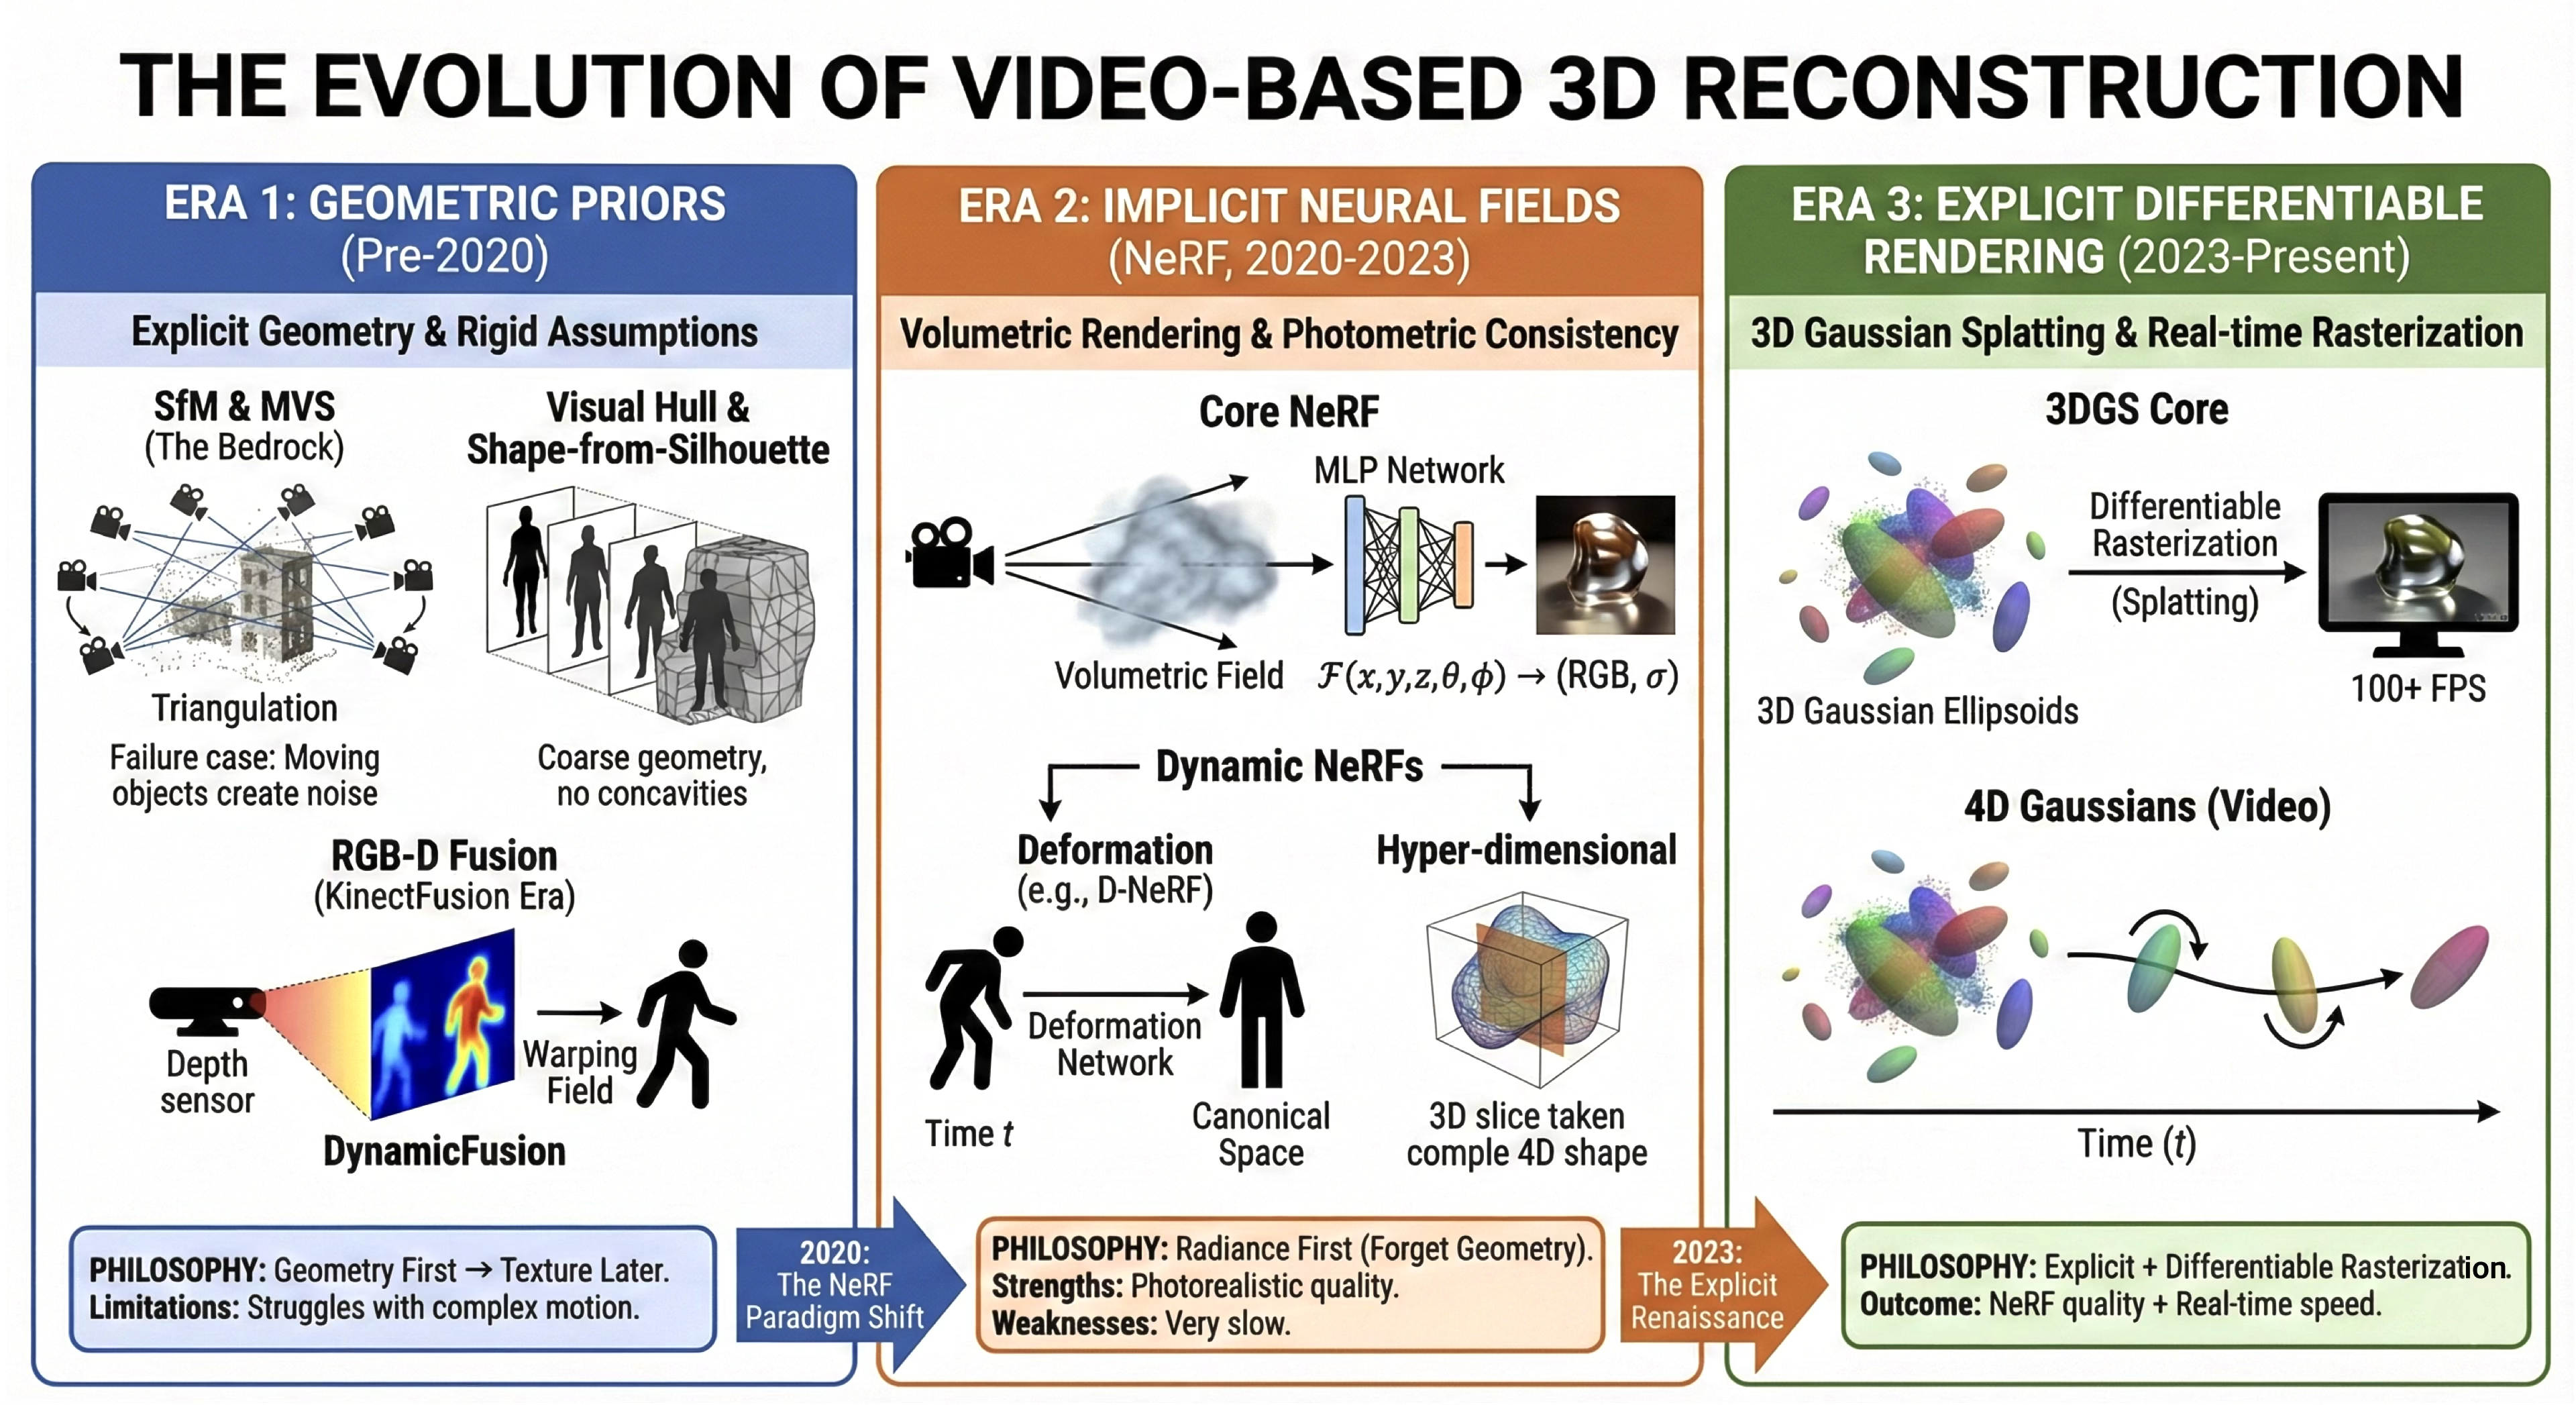
\includegraphics[width=0.95\textwidth]{./img/3d_reconstruction_evolution.png}
  \caption{\textbf{Chronological evolution of dynamic scene modeling.} 
  The timeline illustrates the paradigm shift from \textbf{Implicit Neural Fields} (e.g., D-NeRF, DyNeRF), which prioritize storage efficiency but suffer from slow inference, to \textbf{Hybrid Representations} (e.g., HexPlane) that utilize explicit spatial structures for acceleration, and finally to the emerging \textbf{Explicit Dynamic 3DGS} (e.g., 4D-GS). 
  This trajectory highlights the community's move from continuous MLP-based functions to discrete, rasterizable primitives to achieve real-time rendering capabilities.}
  \label{fig:evolution_3d_reconstruction}
\end{figure*}

%----------------------------------------------------------------------------------------
Recently, \textbf{3D Gaussian Splatting (3DGS)} \cite{gaussian_splatting} has emerged as a compelling alternative, marking a return to explicit volumetric representations. 
By combining the differentiability of deep learning with the efficiency of rasterization-based rendering, 3DGS enables real-time rendering (100+ FPS) and fast training speeds. 
This breakthrough has triggered a new wave of research focused on extending Gaussian primitives to 4D spatiotemporal modeling \cite{4dgs, dynamic3dgs}, aiming to combine the efficiency of explicit representations with the flexibility of neural fields.

Despite the explosion of research papers in this domain, a systematic comparison between the established implicit (NeRF-based) paradigms and the emerging explicit (Gaussian-based) approaches is lacking. 
To fill this gap, this paper provides a structured survey of dynamic scene modeling. Our main contributions are summarized as follows:

\begin{itemize}
  \item \textbf{Structured Taxonomy:} We categorize dynamic modeling methods into four distinct streams: Implicit Deformation Fields (e.g., D-NeRF), Spacetime Neural Fields (e.g., DyNeRF), Hybrid Representations (e.g., HexPlane), and Dynamic Gaussian Splatting (e.g., 4D-GS). This classification clarifies the evolution from continuous functions to discrete primitives.
  
  \item \textbf{Comprehensive Comparison:} We provide an in-depth comparative analysis of these methods, evaluating them not just on visual quality (PSNR/SSIM), but critically on computational efficiency (Training Time, FPS) and storage costs. We highlight the trade-off between the compactness of implicit methods and the speed of explicit methods.
  
  \item \textbf{Future Insights:} We identify critical open challenges, such as the ``baked-in'' lighting limitation and the storage bottleneck of dynamic Gaussians, and propose future directions involving generative AI integration and inverse rendering.
\end{itemize}

%----------------------------------------------------------------------------------------
\section{Preliminaries}
In this section, we first provide a unified mathematical formulation for the problem of video-based 3D reconstruction. 
We then detail the fundamental principles of the two dominant paradigms: the implicit neural representation introduced by NeRF and the explicit differentiable representation proposed by 3D Gaussian Splatting.

%----------------------------------------------------------------------------------------
\subsection{Mathematical Formulation}
Video-based 3D reconstruction can be fundamentally formulated as an inverse rendering problem. 
Given a sequence of $N$ observed images $\mathcal{I} = \{I_1, I_2, \dots, I_N\}$ captured from a video stream, along with their corresponding camera poses $\mathcal{P} = \{P_1, P_2, \dots, P_N\}$ (typically estimated via Structure-from-Motion, SfM), 
the goal is to optimize a 3D scene representation $\mathcal{S}$ such that it can synthesize novel views consistent with the input observations.

Formally, we seek to minimize the photometric reconstruction error between the rendered images and the ground truth images:
\begin{equation}
  \mathcal{S}^* = \mathop{\arg\min}_{\mathcal{S}} \sum_{k=1}^{N} \mathcal{L} \left( \mathcal{R}(\mathcal{S}, P_k), I_k \right)
\end{equation}
where $\mathcal{R}(\cdot)$ denotes the differentiable rendering function that projects the 3D representation $\mathcal{S}$ onto the 2D image plane given a camera pose $P_k$, 
and $\mathcal{L}$ represents the loss function (typically $\ell_1$, $\ell_2$, or D-SSIM) measuring the discrepancy between the synthesized and observed pixels.

%----------------------------------------------------------------------------------------
\subsection{Fundamentals of Neural Radiance Fields}
Neural Radiance Fields (NeRF) represent a scene implicitly as a continuous volumetric function parameterized by a Multi-Layer Perceptron (MLP).

%----------------------------------------------------------------------------------------
\subsubsection{Scene Representation}
The core function, denoted as $F_{\Theta}$, maps a continuous 5D coordinate input---consisting of a 3D spatial location $\mathbf{x} = (x, y, z)$ and
 a 2D viewing direction $\mathbf{d} = (\theta, \phi)$---to a volume density $\sigma$ and a view-dependent emitted color $\mathbf{c} = (r, g, b)$:
\begin{equation}
  F_{\Theta}: (\mathbf{x}, \mathbf{d}) \to (\mathbf{c}, \sigma)
\end{equation}
By conditioning the color on the viewing direction $\mathbf{d}$, NeRF is able to model complex view-dependent effects such as specular reflections.

%----------------------------------------------------------------------------------------
\subsubsection{Volume Rendering Equation}
To synthesize an image, NeRF employs classical volume rendering techniques. 
The color $C(\mathbf{r})$ of a camera ray $\mathbf{r}(t) = \mathbf{o} + t\mathbf{d}$ is computed by integrating the radiance along the ray from near bound $t_n$ to far bound $t_f$:
\begin{equation}
  C(\mathbf{r}) = \int_{t_n}^{t_f} T(t) \sigma(\mathbf{r}(t)) \mathbf{c}(\mathbf{r}(t), \mathbf{d}) \, dt
\end{equation}
where $T(t)$ denotes the accumulated transmittance, representing the probability that the ray travels from $t_n$ to $t$ without hitting any other particles:
\begin{equation}
  T(t) = \exp \left( -\int_{t_n}^{t} \sigma(\mathbf{r}(s)) \, ds \right)
\end{equation}

%----------------------------------------------------------------------------------------
\subsubsection{Discretization}
In practice, the continuous integral is approximated using stratified sampling. The ray is divided into $N$ bins, and the integral is reduced to a finite sum:
\begin{equation}
  \begin{split}
    \hat{C}(\mathbf{r}) &= \sum_{i=1}^{N} T_i (1 - \exp(-\sigma_i \delta_i)) \mathbf{c}_i\,, \\
    & \text{where } T_i = \exp \left( -\sum_{j=1}^{i-1} \sigma_j \delta_j \right)
  \end{split}
\end{equation}
Here, $\delta_i$ is the distance between adjacent samples. This differentiable rendering pipeline allows the MLP parameters $\Theta$ to be optimized via stochastic gradient descent.

%----------------------------------------------------------------------------------------
\subsection{Fundamentals of 3D Gaussian Splatting}
To address the computational inefficiency of volumetric ray-marching in NeRF, 3D Gaussian Splatting (3DGS) introduces an explicit representation based on anisotropic 3D Gaussians, 
enabling real-time rendering via rasterization.

%----------------------------------------------------------------------------------------
\begin{figure}[!t]
  \centering
  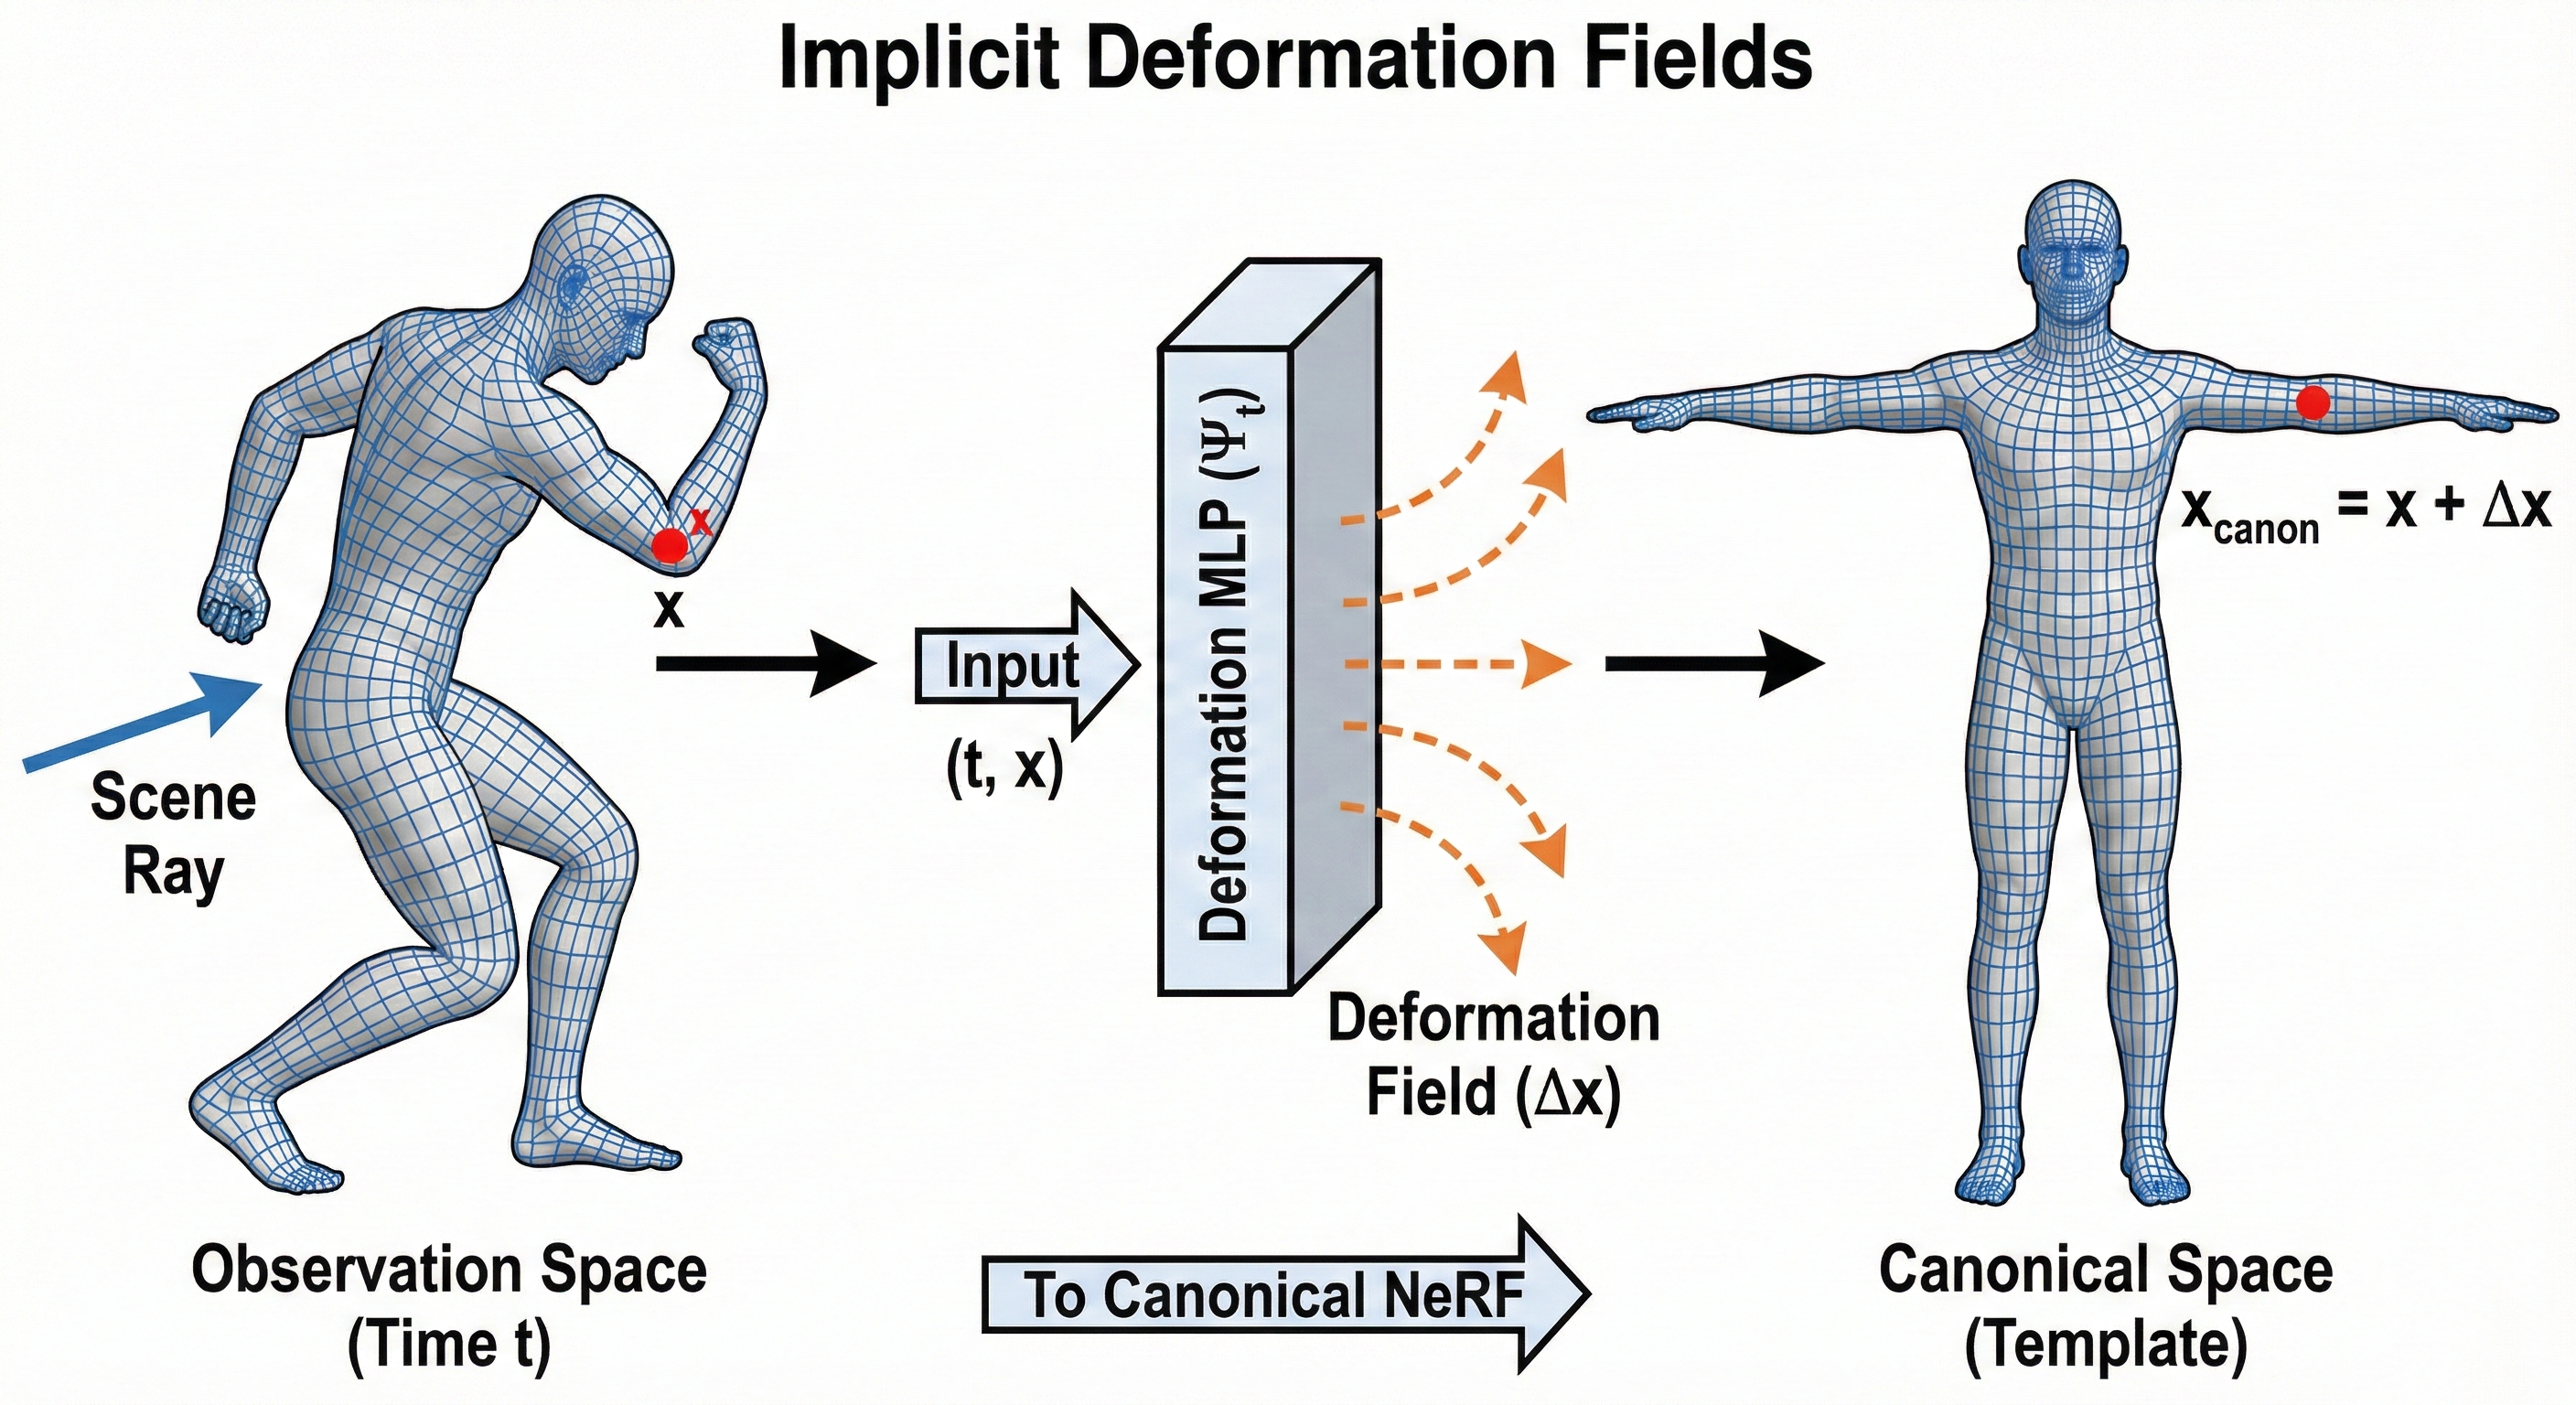
\includegraphics[width=\linewidth]{./img/implicit_deformation_fields.png}
  \caption{Overview of Implicit Deformation Fields. Dynamic scenes are modeled by learning a deformation field that maps points from the observation space to a canonical space, where a static NeRF represents the scene's appearance and geometry.}
  \label{fig:implicit_deformation_fields}
\end{figure}

%----------------------------------------------------------------------------------------
\subsubsection{3D Gaussian Representation}
The scene is represented by a set of 3D Gaussians. Each primitive is defined by a center position $\mu$, a covariance matrix $\Sigma$, an opacity $\alpha$, 
and spherical harmonics (SH) coefficients for view-dependent color. The influence of a Gaussian at a point $\mathbf{x}$ is defined as:
\begin{equation}
  G(\mathbf{x}) = \exp \left( -\frac{1}{2} (\mathbf{x} - \mu)^T \Sigma^{-1} (\mathbf{x} - \mu) \right)
\end{equation}
To ensure the covariance matrix $\Sigma$ remains positive semi-definite during optimization, it is factorized into a scaling matrix $S$ and a rotation matrix $R$:
\begin{equation}
  \Sigma = R S S^T R^T
\end{equation}

%----------------------------------------------------------------------------------------
\subsubsection{Projection and Splatting}
Unlike NeRF's ray-marching, 3DGS projects the 3D Gaussians directly onto the 2D image plane. Given a viewing transformation $W$, the covariance matrix $\Sigma'$ in camera coordinates is approximated as:
\begin{equation}
  \Sigma' = J W \Sigma W^T J^T
\end{equation}
where $J$ is the Jacobian of the affine approximation of the projective transformation. This step effectively ``splats'' the 3D ellipsoids into 2D ellipses.

%----------------------------------------------------------------------------------------
\subsubsection{Tile-based Blending}
The final pixel color is computed using $\alpha$-blending of the $N$ sorted Gaussians overlapping the pixel:
\begin{equation}
  C = \sum_{i \in \mathcal{N}} c_i \alpha_i \prod_{j=1}^{i-1} (1 - \alpha_j)
\end{equation}
Here, $\alpha_i$ is obtained by evaluating the 2D Gaussian multiplied by the learned opacity. 
This tile-based rasterization approach allows for highly efficient backpropagation and real-time rendering speeds ($>100$ FPS), making it particularly suitable for high-resolution video reconstruction.

%----------------------------------------------------------------------------------------
\section{Taxonomy of Dynamic Scene Modeling} % Core

%----------------------------------------------------------------------------------------
\subsection{Implicit Deformation Fields}
This category of methods addresses dynamic scene modeling by decoupling the scene's geometry into two components: a static structure and a time-variant deformation.

%----------------------------------------------------------------------------------------
\subsubsection{Core Assumption and Architecture}
The fundamental assumption of this paradigm is the existence of a time-independent \textbf{Canonical Space}. 
The dynamic scene observed at any time instance $t$ is modeled as a warped version of this canonical configuration \cite{dnerf}. 
This approach simplifies the learning objective by separating motion from appearance.

Architecturally, these frameworks typically employ two joint Multilayer Perceptrons (MLPs):

\textbf{Deformation Network:} This network learns the mapping from the observation space to the canonical space. 
It takes the current 3D position $\mathbf{x}$ and a temporal indicator (time $t$ or a latent code $\omega_i$) as input, and outputs a displacement vector $\Delta \mathbf{x}$ (or a dense vector field).

\textbf{Canonical Network:} This is a standard static NeRF that represents the scene in its ``rest pose''. 
It takes the corrected position $\mathbf{x}_{canon} = \mathbf{x} + \Delta \mathbf{x}$ and viewing direction $\mathbf{d}$ to predict color $\mathbf{c}$ and density $\sigma$.

Mathematically, this process can be formulated as:
\begin{equation}
  (\mathbf{x}_{canon}, \Delta \mathbf{x}) = \mathcal{D}(\mathbf{x}, t), \quad (\mathbf{c}, \sigma) = \mathcal{F}_{\text{NeRF}}(\mathbf{x}_{canon}, \mathbf{d})
\end{equation}
where $\mathcal{D}$ represents the deformation network and $\mathcal{F}_{\text{NeRF}}$ represents the canonical radiance field \cite{dnerf}.

%----------------------------------------------------------------------------------------
\subsubsection{Representative Frameworks}
The evolution of implicit deformation fields can be traced through general-purpose deformations to specialized domain-specific solutions.

\textbf{General Non-Rigid Deformation:}
Pumarola et al. established the baseline with \textbf{D-NeRF}, introducing the translation field $\mathbf{x}(t) \to \mathbf{x}_{canon} + \Delta \mathbf{x}$. 
It optimizes the scene using a sparse set of monocular images, successfully reconstructing objects like a moving mechanical arm or a jumping human \cite{dnerf}.
Addressing the challenges of casual selfie videos (e.g., camera movement), Park et al. introduced \textbf{Nerfies}, which employs learned latent deformation codes $\omega_i$ and \textbf{elastic regularization} to impose rigidity priors, preventing unrealistic distortions in background regions \cite{nerfies}.

\textbf{Handling Topological Changes:}
A critical limitation of continuous deformation fields is their inability to model topological changes (e.g., a mouth opening). 
Park et al. proposed \textbf{HyperNeRF} to address this by lifting the scene into a higher-dimensional ``hyperspace''. 
Instead of simply deforming points, HyperNeRF learns a \textbf{slicing surface} in this ambient hyperspace, effectively modeling topological variations as continuous deformations of the slicing manifold \cite{hypernerf}.

\textbf{Human-Centric Extensions:}
Reconstructing dynamic humans presents unique challenges due to complex articulated motions. Pure deformation fields often fail to capture the kinematic constraints of the human body. 
To address this, \textbf{Neural Body} \cite{neuralbody} incorporates a parametric 3D human model (SMPL) as a geometric prior. It anchors latent codes to the vertices of the deformable mesh, allowing the network to diffuse information across valid poses.
Similarly, \textbf{HumanNeRF} \cite{humannerf} and \textbf{Animatable NeRF} \cite{animatablenerf} introduce skeleton-driven deformation fields, where the warping is explicitly conditioned on the transformation matrices of human bones, enabling high-fidelity re-posing and free-viewpoint rendering of performers.

%----------------------------------------------------------------------------------------
\subsubsection{Summary}

\textbf{Pros}: These methods excel at reconstructing non-rigid, organic objects (such as human faces and bodies) with photorealistic quality. By incorporating domain-specific priors (e.g., SMPL \cite{neuralbody}), they can achieve robust performance even under severe self-occlusion.

\textbf{Cons}: The primary drawback is the computational cost; training is extremely slow due to the MLP queries required for ray marching. 

Furthermore, without explicit topology handling (like HyperNeRF) or skeletal priors, pure deformation fields struggle with large, discontinuous motions.

%----------------------------------------------------------------------------------------
\subsection{Spacetime Neural Fields}
Unlike deformation-based methods that warp a static template, Spacetime Neural Fields treat time as an intrinsic dimension of the scene.
These methods directly learn a continuous function over the spatiotemporal domain, effectively slicing the 4D volume to retrieve the state of the scene at any specific moment.

%----------------------------------------------------------------------------------------
\subsubsection{Core Concepts and Architecture}
The fundamental shift in this paradigm is the expansion of the input domain.
While a standard NeRF maps a 5D coordinate $(\mathbf{x}, \mathbf{d})$ to color and density, Spacetime Neural Fields extend this to a \textbf{Higher-dimensional Input} by incorporating time $t$.
The mapping function evolves into $F_{\Theta}: (\mathbf{x}, \mathbf{d}, t) \to (\mathbf{c}, \sigma)$. To handle complex dynamics, two primary strategies are employed:

\textbf{Latent Code Modulation:} Instead of using a raw scalar $t$, methods like DyNeRF learn a set of compact, time-variant \textit{latent codes} $\mathbf{z}_t$ for each frame.
These codes are fed into the MLP alongside spatial coordinates, acting as a switch that modulates the network's activations to represent topological changes, varying illumination, and transient objects.

\textbf{Physical Consistency (Scene Flow):} To enforce temporal coherence, some approaches incorporate physical constraints.
A notable example is \textbf{NSFF (Neural Scene Flow Fields)} \cite{nsff}, which predicts not only the radiance and density but also the 3D \textit{Scene Flow} vector $\mathbf{f}$.
By enforcing consistency between the backward/forward flow and the geometric positions across frames, the model ensures that the dynamic representation adheres to physical motion laws.

Mathematically, the general formulation for this category can be expressed as:
\begin{equation}
(\mathbf{c}, \sigma) = F_{\Theta}(\mathbf{x}, \mathbf{d}, \mathbf{z}_t) \quad \text{or} \quad (\mathbf{c}, \sigma, \mathbf{f}) = F_{\Theta}(\mathbf{x}, t)
\end{equation}
where $\mathbf{z}_t$ represents the learned latent code and $\mathbf{f}$ denotes the predicted scene flow vector.

%----------------------------------------------------------------------------------------
\subsubsection{Representative Frameworks}
In the following, we discuss two representative frameworks that address dynamic modeling under distinct input constraints: \textbf{DyNeRF} for synchronized multi-view videos and \textbf{Video-NeRF} for casual monocular captures.

%----------------------------------------------------------------------------------------
\begin{figure}[!t]
  \centering
  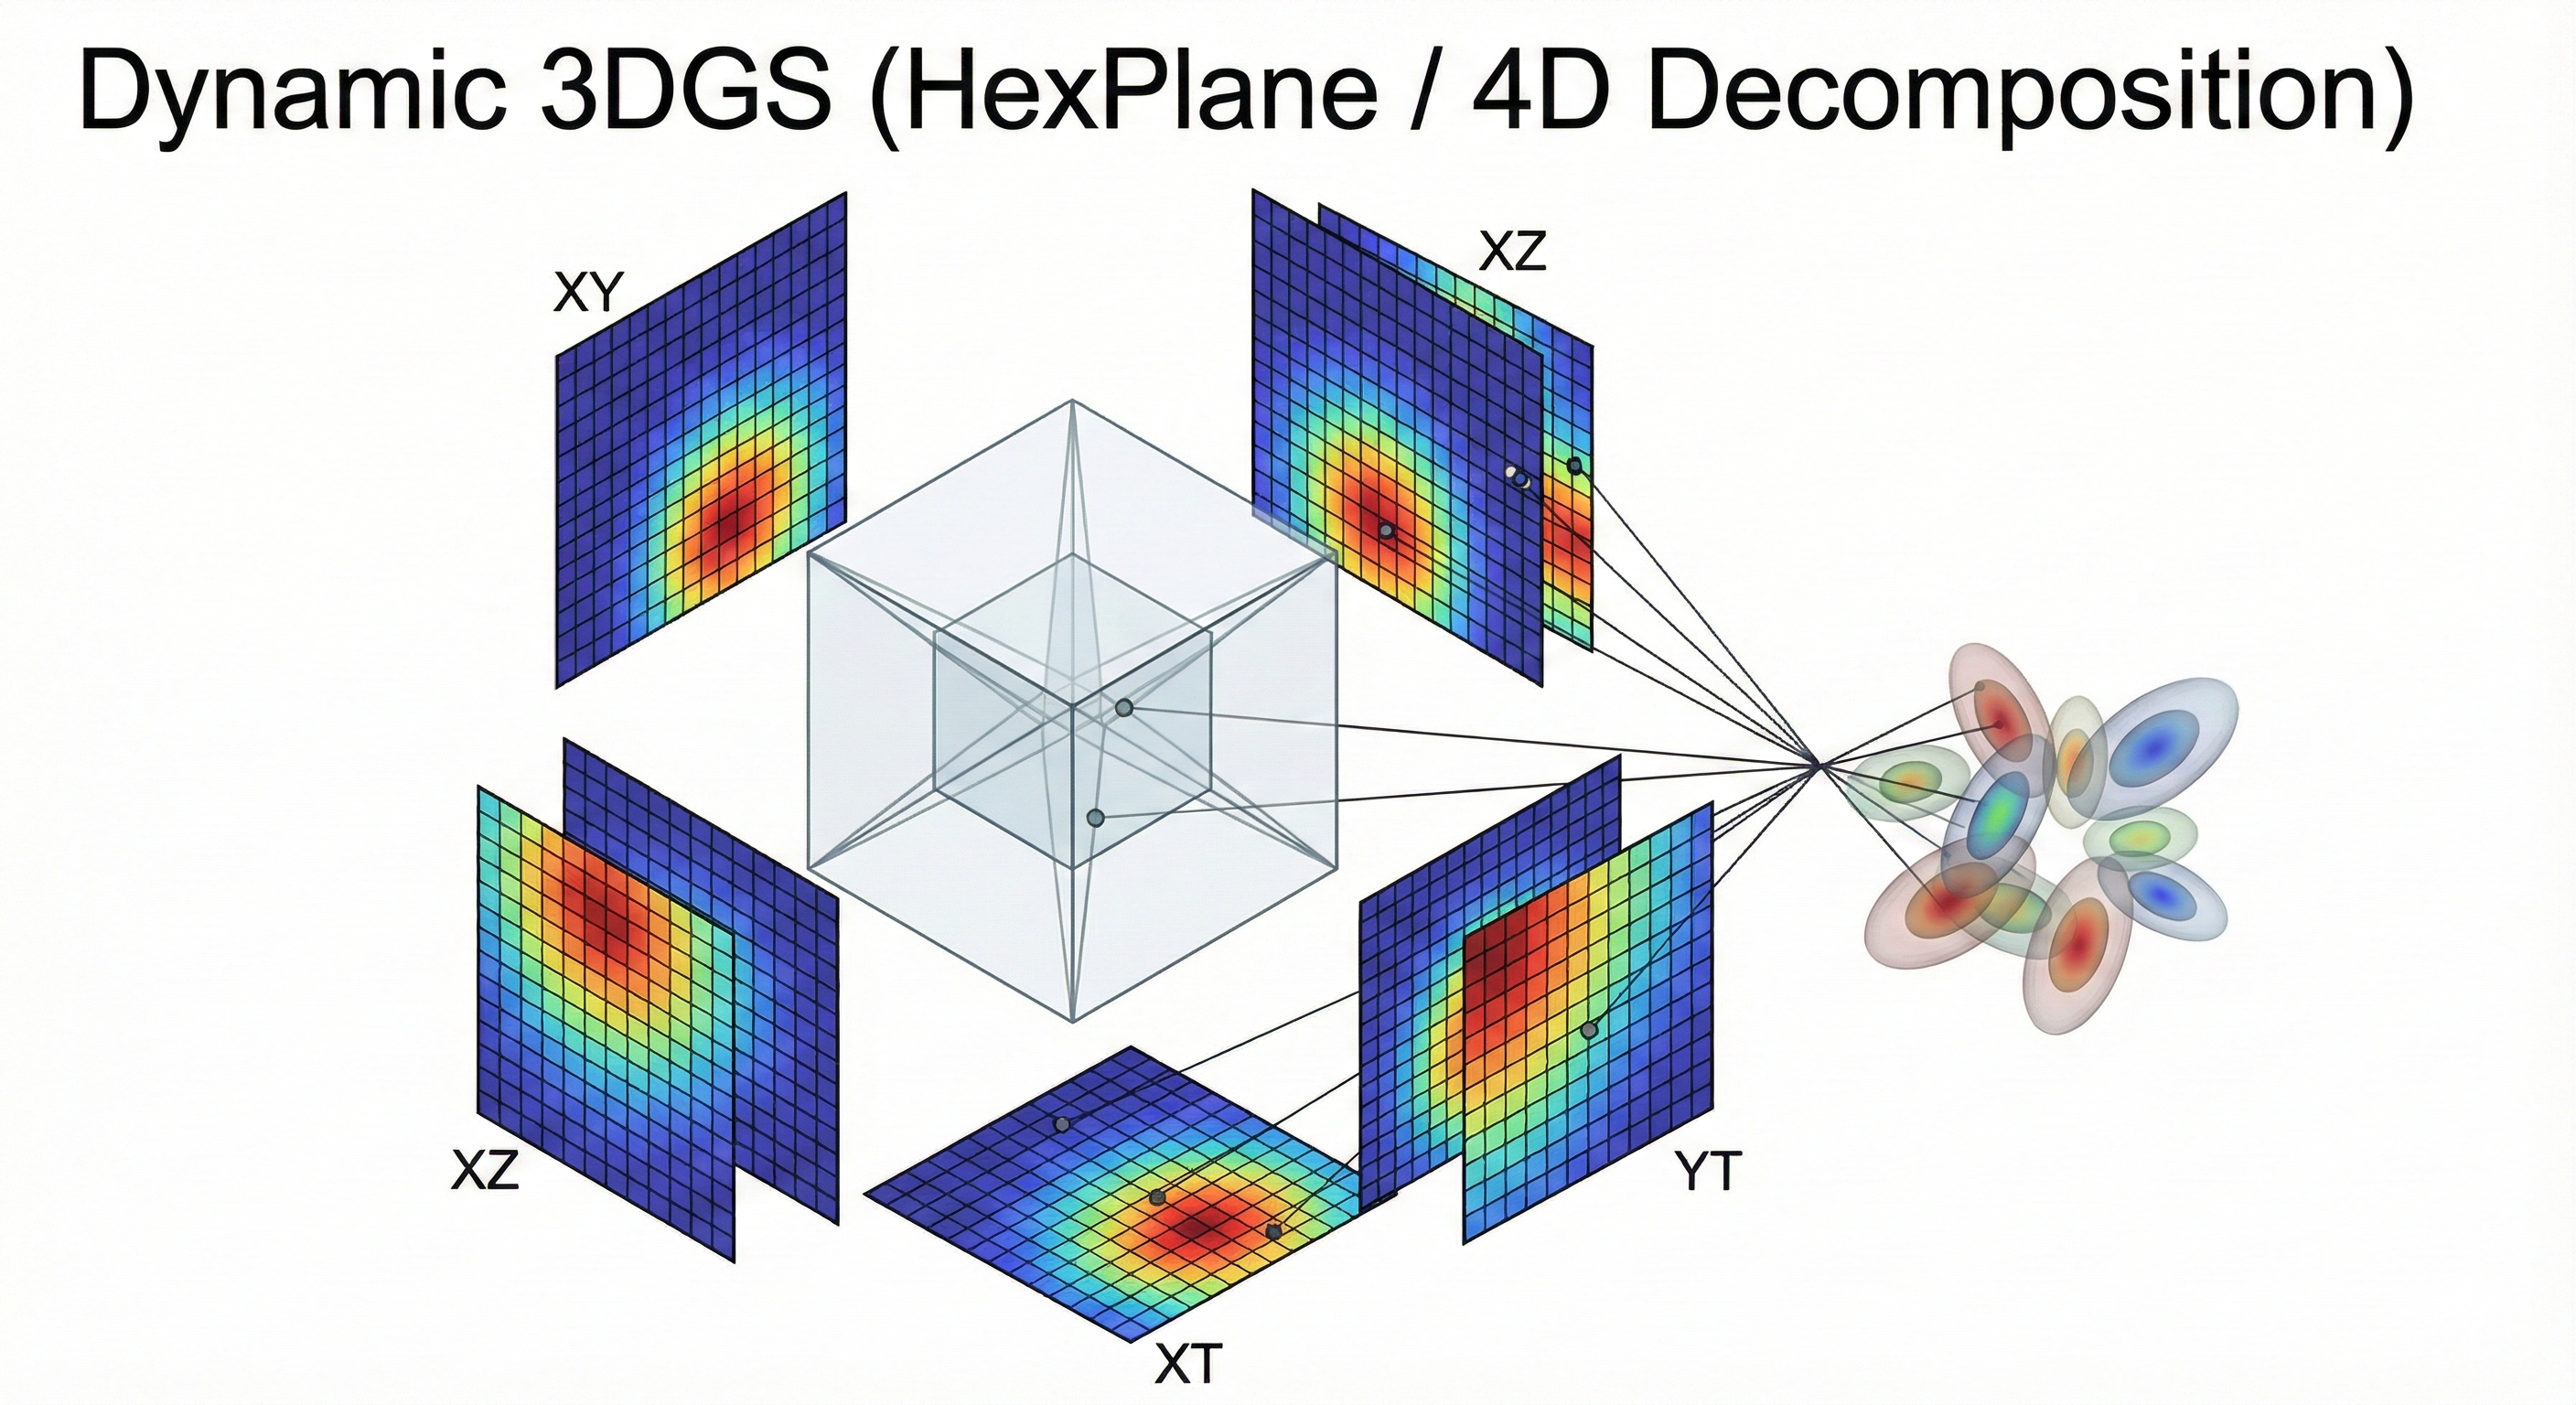
\includegraphics[width=\linewidth]{./img/dynamic_gs.png}
  \caption{Overview of Dynamic Gaussian Splatting. Dynamic scenes are modeled by extending 3D Gaussians with temporal parameterization, either via deformation from a canonical set or direct 4D spatiotemporal representation.}
  \label{fig:dynamic_gaussian_splatting}
\end{figure}

%----------------------------------------------------------------------------------------
\textbf{DyNeRF (Dynamic NeRF):} Li et al. proposed DyNeRF to address the challenge of reconstructing dynamic scenes from multi-view videos \cite{dynerf}.
Instead of a deformation field, DyNeRF conditions the radiance field on a learnable latent embedding $\mathbf{z}_t$. This allows the model to capture complex dynamics that are difficult to model with continuous deformations, such as flame, pouring liquid (topology changes), and view-dependent lighting effects.

\textbf{Video-NeRF:} Focusing on the challenging monocular setting, Video-NeRF learns a direct mapping from spacetime coordinates $(\mathbf{x}, t)$ to an irradiance field (omitting view dependence to handle single-video ambiguity).
To prevent the ``motion-appearance ambiguity'' (where geometry changes are incorrectly explained as texture changes), it incorporates depth supervision from pre-trained monocular estimators and introduces a ``static scene loss'' to constrain unobserved regions by propagating information across time \cite{video_nerf}.

%----------------------------------------------------------------------------------------
\subsubsection{Summary}

\textbf{Pros:} These methods are well-suited for large-scale scenes and complex dynamics involving drastic topological changes (e.g., fluid dynamics, fire) where defining a canonical template is infeasible.

\textbf{Cons:} The addition of the time dimension significantly expands the sampling space, leading to the ``curse of dimensionality''. Without sufficient data (e.g., multi-view rigs) or strong regularization (e.g., depth/flow priors), these models are prone to overfitting or producing temporally incoherent artifacts.

%----------------------------------------------------------------------------------------
\subsection{Dynamic Gaussian Splatting}
This category represents the current state-of-the-art (SOTA), marking a shift from implicit neural fields back to explicit, rasterizable primitives. By extending 3D Gaussian Splatting (3DGS) to the temporal domain, these methods aim to combine the photorealism of NeRF with the real-time rendering capabilities of rasterization.

%----------------------------------------------------------------------------------------
\subsubsection{Core Concepts and Architecture}
The fundamental primitive in this paradigm is the \textbf{3D Gaussian}, characterized by a center position $\mu$, a covariance matrix $\Sigma$, an opacity $\alpha$, and spherical harmonics (SH) for color. To ensure physical validity, the covariance is factorized into scaling $S$ and rotation $R$ matrices: $\Sigma = R S S^T R^T$.

To handle dynamic scenes without incurring the prohibitive memory cost of storing per-frame Gaussians, the core strategy is \textbf{Temporal Parameterization}. The attributes of Gaussians are modeled as functions of time $t$. The influence of a dynamic Gaussian at time $t$ is formulated as:
\begin{equation}
    G(\mathbf{x}, t) = \exp \left( -\frac{1}{2} (\mathbf{x} - \mu(t))^T \Sigma(t)^{-1} (\mathbf{x} - \mu(t)) \right)
\end{equation}
where $\mu(t)$ and $\Sigma(t)$ denote time-variant position and covariance. Two primary streams exist to model these functions:

\textbf{Deformation-based Approach:} Similar to D-NeRF, this stream maintains a set of static \textit{Canonical Gaussians}. A learnable deformation network predicts offsets for position, rotation, and scaling ($\delta x, \delta r, \delta s$) to warp canonical primitives to the current timestamp.

\textbf{4D Spacetime Primitives:} Alternatively, the scene can be represented holistically by querying a high-dimensional feature space. Techniques like \textbf{HexPlane decomposition} factorize the 4D spatiotemporal volume into multi-resolution 2D planes (e.g., $xy, xt, yt$) to efficiently encode temporal dynamics.

%----------------------------------------------------------------------------------------
\subsubsection{Representative Frameworks}
In the following, we discuss two representative frameworks that implement these strategies: \textbf{Deformable 3DGS} for the deformation-based stream and \textbf{4D-GS} for the spatiotemporal representation.

\textbf{Deformable 3DGS:} Yang et al. proposed a framework that learns 3D Gaussians in a canonical space coupled with a deformation field. Unlike NeRF-based deformations that only modify positions, Deformable 3DGS explicitly predicts offsets for position, rotation, and scaling ($\delta x, \delta r, \delta s$) to ensure the ellipsoids align correctly with surface motion. It also introduces an ``annealing smooth training'' mechanism to mitigate temporal jitter caused by inaccurate poses in real-world datasets \cite{deformable_3dgs}.

\textbf{4D-GS:} Wu et al. introduced a holistic representation combining 3D Gaussians with 4D neural voxels. To solve the memory bottleneck, they utilize a \textbf{HexPlane} structure to encode spatial-temporal features. A lightweight multi-head decoder then predicts the Gaussian deformations from these features. This design enables real-time rendering (e.g., 82 FPS at $800 \times 800$ resolution) while maintaining compact storage comparable to static methods \cite{4dgs}.

%----------------------------------------------------------------------------------------
\subsubsection{Summary}

\textbf{Pros:} These methods inherit the efficiency of the rasterization pipeline, achieving real-time rendering speeds ($>30$ FPS) and fast training convergence (often within minutes), which addresses the primary limitation of implicit NeRFs \cite{4dgs}.

\textbf{Cons:} They can be memory-intensive (high VRAM usage) when the number of primitives grows large. Furthermore, modeling large, complex motions from monocular video remains challenging, potentially leading to overfitting or artifacts in unseen views \cite{deformable_3dgs}.

%----------------------------------------------------------------------------------------
\subsection{Hybrid and Accelerated Representations}

While implicit deformation fields offer high fidelity and spacetime neural fields handle complex topology, both suffer from slow training and inference speeds due to the heavy reliance on large MLPs. 
Hybrid representations address this bottleneck by combining \textbf{explicit spatial data structures} (to store learnable features) with \textbf{lightweight implicit decoders} (to interpret them). 
This paradigm serves as a crucial bridge between pure NeRFs and the fully explicit 3DGS.

%----------------------------------------------------------------------------------------
\subsubsection{Core Strategy: Spatial Acceleration}
The core insight of this category is to replace the ``deep'' computation of a large MLP with a ``shallow'' lookup operation. 
Instead of mapping a coordinate $\mathbf{x}$ directly to color/density via a deep network, hybrid methods first query a learnable feature vector $\mathbf{f}$ from a spatial structure (e.g., Voxel Grid, Octree, or Hash Table) and then pass this feature to a tiny MLP:
\begin{equation}
    \mathbf{f} = \text{Query}(\mathcal{S}, \mathbf{x}), \quad (\mathbf{c}, \sigma) = \text{MLP}_{\text{tiny}}(\mathbf{f})
\end{equation}
where $\mathcal{S}$ represents the explicit data structure. This design significantly reduces the floating-point operations (FLOPs) required per sample.

%----------------------------------------------------------------------------------------
\subsubsection{Representative Frameworks}
In the following, we discuss four milestone frameworks that utilize distinct spatial data structures---ranging from hash grids and tensor decomposition to sparse voxels and point clouds---to achieve computational efficiency.

\textbf{Instant-NGP:} Müller et al. revolutionized the field with \textit{Instant Neural Graphics Primitives}, which introduced \textbf{Multiresolution Hash Encoding}. 
By mapping spatial coordinates to a set of learnable feature vectors stored in hash tables at multiple resolution levels, Instant-NGP reduces the training time of radiance fields from hours to seconds. 
Although originally static, its hash encoding backbone has become the standard component for accelerating dynamic methods (including many Spacetime NeRFs and Dynamic 3DGS variants) \cite{instant_ngp}.

\textbf{TensoRF \& K-Planes:} To handle the high memory footprint of dense voxel grids (which scale cubically $O(N^3)$), these methods employ \textbf{Tensor Decomposition}. 
TensoRF factorizes the 3D scene tensor into vector-matrix outer products. 
Extending this to dynamic scenes, \textbf{K-Planes} decomposes the 4D spatiotemporal volume into six planar planes (e.g., $xy, xt, yt$). 
This decomposition allows for explicit modeling of time while maintaining a low memory footprint, effectively ``unrolling'' the complex dynamic scene into manageable 2D feature maps \cite{tensorf, kplanes}.

\textbf{Plenoxels:} Taking the ``hybrid'' concept to its limit, Fridovich-Keil et al. proposed \textit{Plenoxels}, which eliminates the neural network entirely. 
It optimizes a sparse voxel grid where each voxel stores spherical harmonics coefficients directly. 
This work demonstrated that the photorealism of NeRF stems primarily from the differentiable volumetric rendering formulation rather than the neural network itself \cite{plenoxels}.

\textbf{Point-NeRF:} While grid-based methods offer speed, they struggle with empty space inefficiency. 
Xu et al. proposed \textit{Point-NeRF}, which combines accurate 3D point clouds (from MVS) with neural radiance fields. 
Instead of querying a dense grid, Point-NeRF stores neural features on discrete points. 
During ray-marching, features are aggregated from nearby points to predict radiance. 
This approach effectively skips empty space and serves as a significant precursor to 3DGS, demonstrating the potential of point-based neural rendering \cite{point_nerf}.

%----------------------------------------------------------------------------------------
\subsubsection{Summary}

\textbf{Pros:} These methods offer a superior balance between speed and quality. Training is orders of magnitude faster than pure MLP-based NeRFs, and inference is often real-time or near real-time.

\textbf{Cons:} They typically consume more memory (VRAM) than compact pure-implicit models. Additionally, implementing efficient CUDA kernels for hash lookups or sparse grids is technically more complex than standard MLPs.

%----------------------------------------------------------------------------------------
\section{Datasets and Metrics}

%----------------------------------------------------------------------------------------
\subsection{Common Datasets}
To evaluate the performance of dynamic scene modeling algorithms, various datasets have been proposed, ranging from controlled synthetic environments to complex real-world captures. 
We categorize the mainstream datasets into synthetic and real-world collections.

%----------------------------------------------------------------------------------------
\subsubsection{Synthetic Datasets}
\textbf{D-NeRF Dataset} --- Pumarola et al. introduced this dataset as a standard benchmark for monocular dynamic view synthesis. 
It consists of 8 synthetic scenes generated using physically-based rendering. The scenes exhibit diverse motion patterns, categorized into:
\begin{itemize}
  \item \textbf{Articulated Motion:} \textit{T-Rex, Lego, Tractor}.
  \item \textbf{Non-rigid / Deformable Motion:} \textit{Hell Warrior, Mutant, Hook, Stand Up, Jumping Jacks}.
  \item \textbf{Topological Changes:} \textit{Bouncing Balls}.
\end{itemize}
Since it provides perfect camera poses and ground truth depth, it serves as the primary testbed for validating deformation accuracy and rendering quality without the interference of pose errors errors\footnote{D-NeRF dataset available at: \url{https://www.albertpumarola.com/research/D-NeRF/index.html}}.

%----------------------------------------------------------------------------------------
\subsubsection{Real-world Datasets}
\textbf{Neural 3D Video (N3V) Dataset} --- Proposed by Li et al. (DyNeRF), this dataset focuses on high-fidelity reconstruction from synchronized \textbf{multi-view} videos (typically 18-21 cameras). 
Recorded at 2.7K resolution and 30 FPS, it features challenging indoor scenarios with complex illumination and volumetric effects. 
Representative scenes include \textit{Flame Salmon} (fire/smoke), \textit{Coffee Martini} (liquid/reflections), \textit{Cook Spinach} (steam), and \textit{Cut Roasted Beef} (texture changes). 
This dataset is widely used to evaluate methods targeting immersive video and photo-realistic rendering of complex materials\footnote{N3D dataset available at: \url{https://github.com/facebookresearch/Neural_3D_Video}}.

%----------------------------------------------------------------------------------------
\renewcommand{\arraystretch}{1.3}
\begin{table}[H]
  \centering
  \caption{Summary of Common Datasets for Dynamic Scene Modeling}
  \begin{tabularx}{\linewidth}{l|c|c|X}
    \hline
    \textbf{Dataset} & \textbf{Type} & \textbf{Cameras} & \textbf{Key Challenges} \\
    \hline
    D-NeRF \cite{dnerf} & Synthetic & Monocular & Large deformations, Articulated motion \\
    N3V (DyNeRF) \cite{dynerf} & Real & Multi-view & Fire, Smoke, Reflections, High-res \\
    HyperNeRF \cite{hypernerf} & Real & Monocular & Topological changes, Casual capture \\
    Technicolor & Real & Multi-view & Studio quality, Human performance \\
    \hline
  \end{tabularx}
\end{table}

%----------------------------------------------------------------------------------------
\textbf{HyperNeRF Dataset} --- To address the limitation of deformation fields in handling topological changes, Park et al. collected this dataset using casually captured \textbf{monocular} videos. 
It emphasizes ``topologically varying'' objects where standard deformation fields fail. 
Key scenes include \textit{3D Printer} (appearing/disappearing materials), \textit{Broom} (bristles spreading), \textit{Chicken} (elastic deformation), and \textit{Peel Banana} (separation of geometry). 
It also provides a ``Validation Rig'' subset for quantitative evaluation\footnote{HyperNeRF dataset available at: \url{https://hypernerf.github.io}}.

\textbf{Technicolor Light Field Dataset} --- Originally designed for light field research, this dataset contains high-quality multi-view video sequences captured in a studio setting with a 4x4 camera rig. 
Scenes such as \textit{Fabien}, \textit{Painter}, and \textit{Birthday} involve human performances and are frequently used to benchmark hybrid and explicit representations for free-viewpoint video\footnote{Technicolor dataset available at: \url{https://www.interdigital.com/data_sets/light-field-dataset}}.

%----------------------------------------------------------------------------------------
\subsection{Evaluation Metrics}
To quantitatively assess the performance of dynamic scene modeling methods, the community relies on a set of standard metrics covering reconstruction quality, perceptual fidelity, and computational efficiency.

%----------------------------------------------------------------------------------------
\begin{table*}[t]
  \centering
  \caption{\textbf{Quantitative Comparison of State-of-the-Art Methods.} We report average metrics across standard test sets. \textbf{Class} denotes the method category: \textcolor{BlueViolet}{Imp.} (Implicit), \textcolor{OliveGreen}{Hyb.} (Hybrid), and \textcolor{BrickRed}{Exp.} (Explicit). Best results are highlighted in \textbf{bold}, and second best are \underline{underlined}.}
  \label{tab:quantitative_comparison}
  \renewcommand{\arraystretch}{1.2}
  \setlength{\tabcolsep}{6pt}
  \begin{tabular}{l|l|c|ccc|cc|c}
    \hline
    \multirow{2}{*}{\textbf{Method}} & \multirow{2}{*}{\textbf{Class}} & \multirow{2}{*}{\textbf{Year}} & \multicolumn{3}{c|}{\textbf{Rendering Quality}} & \multicolumn{2}{c|}{\textbf{Efficiency}} & \textbf{Storage} \\
    & & & PSNR $\uparrow$ & SSIM $\uparrow$ & LPIPS $\downarrow$ & FPS $\uparrow$ & Train Time $\downarrow$ & Size (MB) \\
    \hline
    \multicolumn{9}{c}{\textit{Dataset: D-NeRF Synthetic (Monocular, $800 \times 800$)}} \\
    \hline
    D-NeRF \cite{dnerf} & \textcolor{BlueViolet}{Imp.} & 2021 & 30.31 & 0.96 & 0.039 & $<$ 1 & $\sim$ 2 days & \textbf{$<$ 5} \\
    TiNeuVox \cite{tineuvox} & \textcolor{OliveGreen}{Hyb.} & 2022 & 32.67 & 0.97 & 0.040 & 1.5 & 28 min & 48 \\
    HexPlane \cite{hexplane} & \textcolor{OliveGreen}{Hyb.} & 2023 & 31.04 & 0.97 & 0.040 & 2.5 & 11 min & 38 \\
    K-Planes \cite{kplanes} & \textcolor{OliveGreen}{Hyb.} & 2023 & 31.61 & 0.97 & 0.038 & 0.9 & 52 min & 418 \\
    \textbf{Deformable 3DGS} \cite{deformable_3dgs} & \textcolor{BrickRed}{Exp.} & 2024 & \underline{33.07} & \underline{0.98} & \textbf{0.018} & \underline{45} & \textbf{$<$ 10 min} & $\sim$ 20 \\
    \textbf{4D-GS} \cite{4dgs} & \textcolor{BrickRed}{Exp.} & 2024 & \textbf{34.05} & \textbf{0.98} & \underline{0.020} & \textbf{82} & \underline{8 min} & \underline{18} \\
    \hline
    \multicolumn{9}{c}{\textit{Dataset: HyperNeRF / N3V (Real-world, various resolutions)}} \\
    \hline
    Nerfies \cite{nerfies} & \textcolor{BlueViolet}{Imp.} & 2021 & 22.20 & 0.80 & 0.193 & $<$ 1 & $\sim$ 16 hours & \textbf{$<$ 10} \\
    HyperNeRF \cite{hypernerf} & \textcolor{BlueViolet}{Imp.} & 2021 & 22.40 & 0.81 & 0.185 & $<$ 1 & $\sim$ 32 hours & \textbf{$<$ 10} \\
    DyNeRF \cite{dynerf} & \textcolor{BlueViolet}{Imp.} & 2022 & 29.58 & 0.92 & 0.098 & $<$ 1 & $\sim$ 1 week & 28 \\
    HexPlane \cite{hexplane} & \textcolor{OliveGreen}{Hyb.} & 2023 & \underline{31.70} & \textbf{0.95} & 0.075 & 0.2 & 12 hours & 250 \\
    \textbf{4D-GS} \cite{4dgs} & \textcolor{BrickRed}{Exp.} & 2024 & 31.15 & \underline{0.94} & \textbf{0.049} & \textbf{30} & \textbf{40 min} & 90 \\
    \hline
  \end{tabular}
\end{table*}

%----------------------------------------------------------------------------------------
\subsubsection{Reconstruction Quality Metrics}
The quality of novel view synthesis is typically assessed using standard image quality assessment (IQA) metrics. 
These metrics evaluate the pixel-level fidelity and perceptual similarity between the rendered images and ground truth references.

\textbf{Peak Signal-to-Noise Ratio (PSNR):} PSNR is the most widely used metric for measuring pixel-level reconstruction accuracy. 
It calculates the ratio between the maximum possible power of a signal and the power of corrupting noise, expressed in decibels (dB):
\begin{equation}
    \text{PSNR} = 10 \cdot \log_{10} \left( \frac{\text{MAX}_I^2}{\text{MSE}} \right)
\end{equation}
where $\text{MAX}_I$ is the maximum pixel value (e.g., 255) and MSE is the Mean Squared Error between the rendered and ground truth images. 
While high PSNR indicates low pixel error, it often favors smooth/blurry results over sharp but slightly misaligned textures.

\textbf{Structural Similarity Index (SSIM):} Unlike PSNR, SSIM measures the structural similarity between two images, 
which correlates better with the human visual system's sensitivity to structural information. It considers luminance, contrast, and structure:
\begin{equation}
    \text{SSIM}(x, y) = \frac{(2\mu_x\mu_y + C_1)(2\sigma_{xy} + C_2)}{(\mu_x^2 + \mu_y^2 + C_1)(\sigma_x^2 + \sigma_y^2 + C_2)}
\end{equation}
where $\mu$ and $\sigma$ represent the mean and variance of image windows. SSIM values range from -1 to 1, with 1 indicating perfect similarity.

\textbf{Learned Perceptual Image Patch Similarity (LPIPS):} Standard metrics (PSNR/SSIM) often fail to capture high-frequency details and perceptual quality. 
LPIPS measures the distance between image patches in the deep feature space of a pre-trained network (e.g., VGG or AlexNet). 
Lower LPIPS scores indicate better perceptual quality, aligning more closely with human judgment, especially for dynamic scenes where slight motion misalignments penalize PSNR heavily but look plausible to humans.

%----------------------------------------------------------------------------------------
\subsubsection{Efficiency Metrics}
In addition to visual quality, the computational efficiency of a method determines its practicality for real-time applications (such as VR/AR) and its scalability for large datasets.

\textbf{Frames Per Second (FPS):} This metric evaluates the inference/rendering speed. 
For real-time applications (VR/AR), a method typically needs to achieve $\ge 30$ FPS. 
Explicit methods like 3DGS often reach 100+ FPS, while implicit NeRFs may struggle at $<1$ FPS.

\textbf{Training Time:} This measures the duration required to optimize the scene representation from scratch. 
It is a critical factor for scalability. Recent Gaussian-based methods have reduced training time from days (D-NeRF) to minutes (4D-GS).

%----------------------------------------------------------------------------------------
\section{Comparative Analysis}
In this section, we provide a systematic comparison of the representative methods discussed in Section III. We evaluate them based on quantitative reconstruction quality, computational efficiency, and storage requirements.

%----------------------------------------------------------------------------------------
\subsection{Quantitative Benchmarks}
Table \ref{tab:quantitative_comparison} summarizes the performance of Implicit (NeRF-based), Hybrid, and Explicit (Gaussian-based) frameworks across standard benchmarks. The comparison is divided into synthetic scenes (D-NeRF dataset) and complex real-world scenes (HyperNeRF and N3V datasets).

%----------------------------------------------------------------------------------------
\subsubsection{Quality vs. Efficiency Trade-off}
The benchmarks reveal a clear paradigm shift. 
Implicit methods (e.g., D-NeRF, HyperNeRF) produce high-fidelity results with extremely compact storage (typically $<10$ MB) due to the spectral bias of MLPs. However, their inference speed is prohibitively slow ($<1$ FPS) for interactive applications. 
Hybrid methods (e.g., HexPlane, TiNeuVox) significantly reduce training time to minutes by utilizing explicit spatial structures, yet their rendering speed remains limited by the ray-marching/accumulation step.

Explicit Gaussian-based methods (Deformable 3DGS, 4D-GS) break this bottleneck. 
As shown in Table \ref{tab:quantitative_comparison}, \textbf{4D-GS} achieves real-time performance (82 FPS on synthetic data, 30 FPS on high-res real data) while matching or surpassing the PSNR/SSIM of offline implicit methods. 
This efficiency gain comes from replacing costly volumetric sampling with rasterization. 
However, this comes at the cost of increased storage requirements (often $2\times$ to $10\times$ larger than implicit models) to store millions of Gaussian primitives.

%----------------------------------------------------------------------------------------
\subsection{Qualitative Visual Comparisons}
While quantitative metrics provide a numerical ranking, they often fail to capture perceptual artifacts such as ghosting, over-smoothing, or geometric distortion. 
In Figure \ref{fig:qualitative_comparison}, we provide a visual comparison of representative methods across three challenging scenarios: topological changes, fine geometric structures, and rapid motion.

%----------------------------------------------------------------------------------------
\begin{figure*}[t]
    \centering
    \includegraphics[width=0.95\textwidth]{./img/qualitative_comparison_composite.png}
    
    \caption{\textbf{Qualitative comparison on challenging scenarios.} 
    \textbf{Left:} Handling topological changes. Deformation fields (Nerfies) cause stretching artifacts, while HyperNeRF handles discontinuities correctly \cite{hypernerf}.
    \textbf{Top Right:} Reconstructing fine details. Implicit methods (TiNeuVox) tend to smooth out thin structures, whereas explicit Deformable 3DGS preserves sharp geometry \cite{deformable_3dgs}.
    \textbf{Bottom Right:} Handling rapid motion. Basic temporal conditioning leads to ghosting (NeRF-T), while latent-conditioned methods (DyNeRF) recover sharp dynamics \cite{dynerf}.}
    \label{fig:qualitative_comparison}
\end{figure*}

%----------------------------------------------------------------------------------------
\subsubsection{Topological Adaptability}
Implicit deformation fields (e.g., Nerfies) rely on continuous mapping functions, which inherently struggle with discontinuous motions. 
As shown in the \textbf{left panel} of Figure \ref{fig:qualitative_comparison}, when representing a splitting object (e.g., opening a mouth or slicing dough), deformation-based methods tend to produce unnatural stretching artifacts. 
In contrast, \textbf{HyperNeRF} successfully handles these topology changes by lifting the deformation into a higher-dimensional hyperspace, allowing for discontinuous slicing \cite{hypernerf}.

\subsubsection{High-Frequency Details}
Explicit representations generally exhibit superior capability in preserving high-frequency details compared to implicit or hybrid fields. 
As illustrated in the \textbf{top right} of Figure \ref{fig:qualitative_comparison} (T-Rex scene), grid-based methods like TiNeuVox often result in over-smoothed geometry due to the limited resolution of the voxel grid or the spectral bias of MLPs. 
\textbf{Deformable 3DGS}, leveraging discrete Gaussian primitives, maintains sharp edges and intricate structures (e.g., the ribs of the skeleton) without blurring \cite{deformable_3dgs}.

\subsubsection{Motion Blur and Ghosting}
Modeling rapid motion from monocular or sparse video remains a significant challenge. 
Naive temporal extensions (e.g., NeRF-T) often fail to disentangle geometry from motion blur, leading to ``ghosting'' artifacts where multiple timestamps appear overlaid. 
As shown in the \textbf{bottom right} of Figure \ref{fig:qualitative_comparison}, methods utilizing compact latent codes (like \textbf{DyNeRF}) demonstrate better temporal consistency, effectively reconstructing sharp appearances even in the presence of fast-moving elements like flames or fluids \cite{dynerf}.

%----------------------------------------------------------------------------------------
\subsection{Efficiency Analysis}
Beyond visual fidelity, the practical deployment of dynamic scene modeling hinges on computational efficiency. 
We analyze the trade-offs across three key dimensions: training convergence, rendering latency, and storage overhead.

%----------------------------------------------------------------------------------------
\subsubsection{Training Efficiency}
Implicit methods (e.g., D-NeRF, DyNeRF) typically require the longest training times (ranging from hours to days) due to the dense sampling required by volumetric ray-marching during backpropagation. 
The global nature of MLPs also makes it difficult to update local regions independently.
Hybrid representations (e.g., TiNeuVox, HexPlane) dramatically accelerate this process (to minutes) by using explicit feature grids that allow for local updates and faster convergence.
Explicit methods (e.g., 4D-GS) further push the boundary, often converging within minutes (e.g., 8 minutes for 4D-GS \cite{4dgs}). 
This speedup is attributed to the rasterization-based pipeline, which avoids expensive volumetric sampling and allows gradients to propagate directly to discrete primitives.

%----------------------------------------------------------------------------------------
\subsubsection{Rendering Speed}
Rendering speed is the primary bottleneck for implicit methods. 
Standard D-NeRF operates at $<1$ FPS due to the necessity of evaluating a deep MLP hundreds of times per ray. 
Hybrid methods improve this by replacing MLP evaluations with feature lookups, achieving interactive rates (1--10 FPS) but often falling short of real-time requirements for high-resolution output.
Explicit Gaussian-based methods demonstrate a decisive advantage here, achieving real-time performance ($30 \sim 100+$ FPS). 
This is achieved by projecting 3D primitives directly onto the 2D screen (splatting), bypassing the ray-marching loop entirely \cite{deformable_3dgs, 4dgs}.

%----------------------------------------------------------------------------------------
\subsubsection{Storage and Memory Footprint}

\textbf{Storage (Disk)} --- Implicit methods are the most storage-efficient, often compressing an entire dynamic sequence into a few megabytes (MB) of MLP weights (e.g., D-NeRF $< 5$ MB). 
Explicit methods, conversely, suffer from a ``curse of storage'' as they need to store millions of Gaussian parameters. 
A naive per-frame 3DGS could consume gigabytes of data. 
However, recent optimized frameworks like 4D-GS reduce this footprint significantly (e.g., $\sim 18$ MB) by using tensor decomposition (HexPlane) to share features across time, making them competitive with compact implicit models \cite{4dgs, dynerf}.

\textbf{Memory (VRAM)} --- During training and inference, explicit and hybrid methods typically consume more GPU memory (VRAM) to store feature grids or point clouds, whereas pure implicit methods have a lower peak memory footprint but higher computational load.

%----------------------------------------------------------------------------------------
\subsubsection{Summary of Trade-offs}

\textbf{For low-storage, offline applications:} Implicit methods (D-NeRF) remain a strong candidate due to their extreme compactness.

\textbf{For real-time applications:} Explicit methods (4D-GS) are currently the only viable option for high-resolution ($>1080$p) real-time rendering.

\textbf{For balanced needs:} Hybrid representations offer a middle ground, providing faster training than pure NeRFs with manageable storage costs.

%----------------------------------------------------------------------------------------
\section{Open Challenges and Future Directions}
Despite the remarkable progress in dynamic scene modeling, several critical challenges remain unresolved. 
In this section, we identify three emerging research directions that are pivotal for the next generation of immersive media.

%----------------------------------------------------------------------------------------
\subsection{Storage Efficiency and Compression}
While explicit methods like 3DGS achieve real-time rendering, they suffer from a high storage footprint compared to implicit MLPs. 
For instance, a naive dynamic 3DGS implementation can consume gigabytes of storage for a short sequence, as it may spawn millions of primitives. 
Although methods like \textbf{4D-GS} utilize HexPlane decomposition to reduce this to $\sim 18$ MB, this is still orders of magnitude larger than standard 2D video codecs (e.g., H.264/HEVC).
\begin{itemize}
    \item \textbf{Challenge:} Developing standard compression algorithms for 4D primitives.
    \item \textbf{Future Direction:} Future work may explore \textbf{Vector Quantization (VQ)} or \textbf{Codebook-based learning} to compress Gaussian attributes (color, rotation, covariance) into discrete indices. Additionally, distinct ``Level of Detail'' (LOD) strategies could be developed to stream dynamic 3D content efficiently over limited bandwidth networks, similar to adaptive bitrate streaming for 2D video.
\end{itemize}

%----------------------------------------------------------------------------------------
\subsection{Handling Long-Duration Videos}
Most current benchmarks (e.g., D-NeRF, N3V) are limited to short clips (typically $< 10$ seconds). Scaling reconstruction to minute-long or hour-long videos presents severe bottlenecks. As noted in \textbf{DyNeRF}, training on a 10-second clip already involves billions of ray samples and significant computational resources.
\begin{itemize}
    \item \textbf{Challenge:} The ``Curse of Dimensionality'' in the temporal axis. Global MLPs struggle to fit long sequences without forgetting (catastrophic forgetting), while explicit methods run out of VRAM.
    \item \textbf{Future Direction:} We envision a shift towards \textbf{Streaming Architectures}. Instead of optimizing a global model for the entire video, future systems might employ a ``sliding window'' approach or keyframe-based residue learning. 
    This would allow the model to reconstruct infinite-length streams by dynamically loading and unloading local spatiotemporal blocks, enabling applications like live volumetric telepresence.
\end{itemize}

%----------------------------------------------------------------------------------------
\subsection{Integration with Generative Models}
The rapid rise of video generation models (e.g., \textbf{Sora}, \textbf{Veo}) has democratized 2D content creation, but these models often lack multi-view consistency and explicit 3D geometry.
\begin{itemize}
    \item \textbf{Challenge:} Bridging the gap between 2D generative priors and 3D/4D reconstruction pipelines.

    \item \textbf{Future Direction:} Dynamic Scene Modeling serves as the ideal ``3D lifting'' mechanism for generative AI. 

        \textbf{Text-to-4D:} Combining text-to-video models with Dynamic 3DGS to generate 4D assets directly from prompts. The explicit nature of Gaussians makes them easier to manipulate than implicit NeRFs.

        \textbf{4D Editing:} Using generative diffusion models to stylize or edit reconstructed 4D scenes (e.g., changing the weather in a captured dynamic video) while maintaining temporal consistency.
\end{itemize}

%----------------------------------------------------------------------------------------
\subsection{Disentanglement and Relighting}
A fundamental limitation of current SOTA methods (including DyNeRF and 3DGS) is the problem of \textbf{``baked-in'' lighting}. 
Existing frameworks typically model the final radiance color $c$ directly via Spherical Harmonics (SH) or latent codes, which entangles the object's surface material properties with the environmental lighting at the time of capture \cite{4dgs, dynerf}.
\begin{itemize}
    \item \textbf{Challenge:} The inability to modify lighting conditions after training. Since shadows and reflections are ``frozen'' into the geometry or texture, moving these objects into a new virtual environment (e.g., in a game engine or Metaverse) results in visual inconsistencies.
    \item \textbf{Future Direction:} The community is moving towards \textbf{Dynamic Inverse Rendering}. This involves decomposing the radiance field into physically based components: geometry, material (BRDF: albedo, roughness), and spatially-varying lighting. Integrating physics-based rendering (PBR) pipelines with dynamic 3DGS will be crucial for achieving editable, relightable 4D assets.
\end{itemize}

%----------------------------------------------------------------------------------------
\section{Conclusion}
In this survey, we have presented a comprehensive taxonomy of dynamic scene modeling, tracing the evolution from implicit deformation fields to the latest explicit 4D Gaussian Splatting techniques. 
We analyzed the trade-offs between different paradigms: 

\textbf{Implicit methods} (e.g., D-NeRF) excel in storage efficiency ($<5$ MB) but suffer from slow training. 

\textbf{Hybrid representations} (e.g., HexPlane) bridge the gap by leveraging spatial data structures for faster convergence. 

\textbf{Explicit methods} (e.g., 4D-GS) have revolutionized the field by enabling real-time rendering ($>80$ FPS) suitable for interactive applications.

However, as discussed in our analysis of open challenges, the journey is far from over. 
Future research must address the bottlenecks of storage compression, long-duration video processing, and the disentanglement of lighting from geometry. 
We believe that the convergence of explicit dynamic representations with generative AI priors will pave the way for the next generation of immersive, editable, and photorealistic 4D content creation.

%----------------------------------------------------------------------------------------
% References
%----------------------------------------------------------------------------------------
\bibliography{reference}

\newpage

%----------------------------------------------------------------------------------------
\section{Biography Section}
\begin{IEEEbiographynophoto}{Yuwei ZHAO}
Use $\backslash${\tt{begin\{IEEEbiographynophoto\}}} and the author name as the argument followed by the biography text.
\end{IEEEbiographynophoto}

%----------------------------------------------------------------------------------------
\end{document}